\documentclass{article}

% if you need to pass options to natbib, use, e.g.:
%     \PassOptionsToPackage{numbers, compress}{natbib}
% before loading neurips_2018

% ready for submission
% \usepackage{neurips_2018}

% to compile a preprint version, e.g., for submission to arXiv, add add the
% [preprint] option:
%     \usepackage[preprint]{neurips_2018}

% to compile a camera-ready version, add the [final] option, e.g.:
     \usepackage[final]{neurips_2018}

% to avoid loading the natbib package, add option nonatbib:
%     \usepackage[nonatbib]{neurips_2018}

\usepackage[utf8]{inputenc} % allow utf-8 input
\usepackage[T1]{fontenc}    % use 8-bit T1 fonts
\usepackage{hyperref}       % hyperlinks
\usepackage{url}            % simple URL typesetting
\usepackage{booktabs}       % professional-quality tables
\usepackage{amsfonts}       % blackboard math symbols
\usepackage{nicefrac}       % compact symbols for 1/2, etc.
\usepackage{microtype}      % microtypography
\usepackage{graphicx}
\usepackage{subfigure}
\title{Sentiment Analysis on Amazon Fine Food Reviews}

% The \author macro works with any number of authors. There are two commands
% used to separate the names and addresses of multiple authors: \And and \AND.
%
% Using \And between authors leaves it to LaTeX to determine where to break the
% lines. Using \AND forces a line break at that point. So, if LaTeX puts 3 of 4
% authors names on the first line, and the last on the second line, try using
% \AND instead of \And before the third author name.

\author{%
  Hanyi Zhang\\
  %
  Yuchen Zeng\\
  %
  Yarong Liu\\
  Stevens Institute of Technology\\
  Hoboken, NJ 07030 \\
  % examples of more authors
  % \And
  % Coauthor \\
  % Affiliation \\
  % Address \\
  % \texttt{email} \\
  % \AND
  % Coauthor \\
  % Affiliation \\
  % Address \\
  % \texttt{email} \\
  % \And
  % Coauthor \\
  % Affiliation \\
  % Address \\
  % \texttt{email} \\
  % \And
  % Coauthor \\
  % Affiliation \\
  % Address \\
  % \texttt{email} \\
}

\begin{document}
% \nipsfinalcopy is no longer used

\maketitle
\begin{abstract}
Nowadays more and more people choose to buy their food online. When they make a decision between similar items, reviews are much more important to them because these text could help them to learn much more information about this item. In our project, we try to use CNN, RNN, KNN and Seq2seq to sentiment analysis on these food reivews.
\end{abstract}
\section{Introduction}
In this project, we find a food reviews dataset from Kaggle. This dataset consists of reviews of fine foods from Amazon. The data span a period of more that 10 years, including all 500000 reviews up to October 2012. Reviews include product ID and user information, ratings of product, time of the review, a plain text reviews and the summary of every text reviews. There are about 568454 reviews, 256059 users, 74258 products and 260 users with 50 reviews. The purpose of this project is to predict the emotion of each reviews.\\[2]
At the beginning, we analyzed the ratings of 35 products in the dataset over the last 10 years. Averaging the ratings of every products in every three months, using the linear regression of 3rd order polynomial and 4th order polynomial to fit the changes of ratings of products.These are the example pictures of two products.

\begin{figure}[htbp]
\centering
\begin{minipage}[t]{0.48\textwidth}
\centering
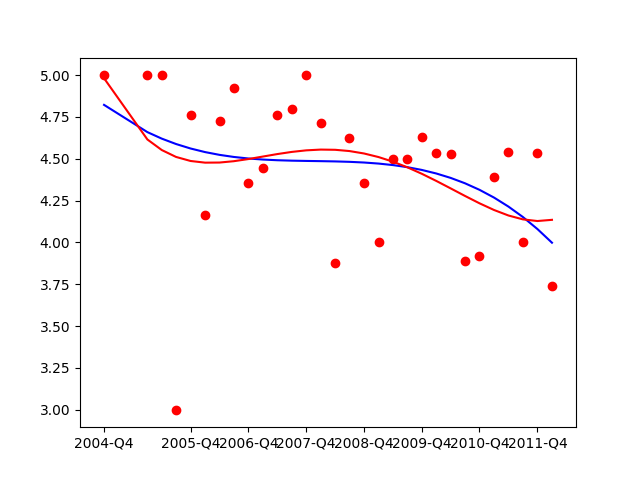
\includegraphics[width=5cm]{Intro-01.png}
\caption{Product-01}
\end{minipage}
\begin{minipage}[t]{0.48\textwidth}
\centering
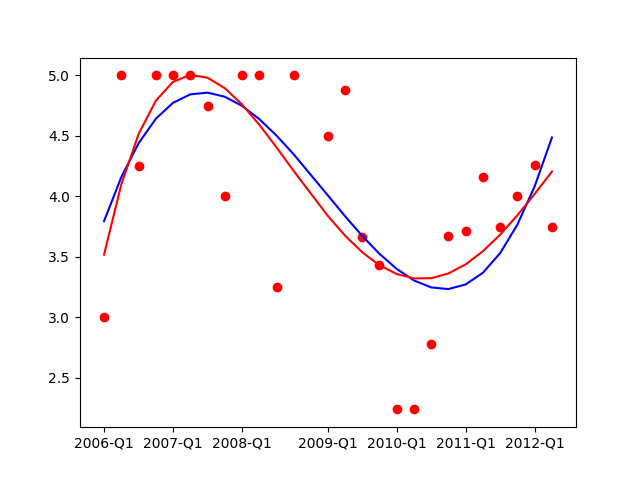
\includegraphics[width=5cm]{Intro-02.png}
\caption{Product-02}
\end{minipage}
\end{figure}

\section{Related Work}
\subsection{Stop Words}
In computer science, stop words are words that are ignored by NLP(Nature language processing). Generally,  stopwords are the most common words in natural language. And there are no universal stop words in NLP tools. These are some of the most common stop words, such as the, is, at, which, and on.  On removing stopwords, dataset size decreases and the time to train the model also decreases. Removing stopwords can potentially help improve the performance as there are fewer and only meaningful tokens left. Thus, it could increase classification accuracy. But on the other hand, removing stopwords will also losing some information.\\[2]
In our project,  we are trying to find out the best stopwords list. We have tested the stopwords list of NLTK, two customized stopwords list, and None stopwords. 

\subsection{Length of input}
During NLP, we need to Pre-processing our data, which are lines of words, and convert it to vectors with the same length. By reducing the length, we can reduce the training time. On the other hand, reducing the length will also result in losing information. \\[2]
In our project, we are trying to find out the best length of vector of each review. And we have chosen the Mean,  Quartile, Medium as vector length.
\subsection{KNN}
KNN( k-nearest neighbors algorithm)  is a non-parametric method used for classification and regression. It was developed from the need to perform discriminant analysis when reliable parametric estimates of probability densities are unknown or difficult to determine. In an unpublished US Air Force School of Aviation Medicine report in 1951, Fix and Hodges introduced a non-parametric method for pattern classification that has since become known as the k-nearest neighbor rule (Fix \& Hodges, 1951).\\[2]
KNN can be used for classification — the output is a class membership (predicts a class — a discrete value). An object is classified by a majority vote of its neighbors, with the object being assigned to the class most common among its k nearest neighbors. It can also be used for regression — output is the value for the object (predicts continuous values). This value is the average (or median) of the values of its k nearest neighbors.\\[2]
The performance of KNN is good in some cases even if it is less complex than CNN or RNN. In our project, We have implemented a KNN Classifier.
\subsection{CNN and RNN}
The most common use for CNN is image classification, for example identifying satellite images that contain roads or classifying hand written letters and digits. There are other quite mainstream tasks such as image segmentation ,signal processing and NLP. In our project, we will use CNN (Convolutional Neural Networks) built by keras to generate sentiment from Amazon reviews.\\[2]
Recurrent Neural Network is a type of Neural Network where the output from previous step are fed as input to the current step. In traditional neural networks, all the inputs and outputs are independent of each other, but in cases like when it is required to predict the next word of a sentence, the previous words are required and hence there is a need to remember the previous words. So, another model we want to use is RNN (Recurrent Neural Network). It is also built by keras.

\subsection{seq2seq}
In order to have better performance, we want to use a seq2seq model. Which means we want to get abstract from different reviews, because some of them  are too long, so no matter CNN and RNN models will receive some redundant information and make a wrong wrong prediction.\\[2]
In our project, we build a Deep Neural Networks which base on the sequence to sequence model which has two RNN parts in it, encoder model and decode model. The goal of encoder model is learn the input text and transfer them into different vectors which can represent the input and can be calculated by computer. Similarly, decoder model's task is translate these vectors into sentences which can be read by human.

\subsection{technique in RNN}
There are many technique which can be used in seq2seq models such as teacher forcing, attention and beam search.\\[2]
Teacher forcing is a method for quickly and efficiently training recurrent neural network models that use the ground truth from a prior time step as input. It is a network training method critical to the development of deep learning language models used in machine translation, text summarization, and image captioning, among many other applications. In our project, we want to find a ratio of teacher forcing which means, some time steps use this technology, other time steps don't use it.\\[2]
Attention is a mechanism that was developed to improve the performance of the Encoder-Decoder RNN on machine translation. And it is proposed as a solution to the limitation of the Encoder-Decoder model encoding the input sequence to one fixed length vector from which to decode each output time step. This issue is believed to be more of a problem when decoding long sequences. In out project, we will implement a global attention model.

\section{Methods}
\subsection{Convolutional Neural Network}
When we process the food reviews, the first thing we should do is using Word Embedding which could map words in the food reviews to vector of real number. Then we can train different kind of models to predict the emotion of each reviews.\\[2]
In order to better introduce CNN, we will use an image as example. When using CNN for text, just change the image matrix to word matrix.
In general, CNN includes two parts: a block of convolutional layers and a block of fully-connected layers, other than that, you can add Dropout layer if required. 
\begin{figure}[htbp]
\centering
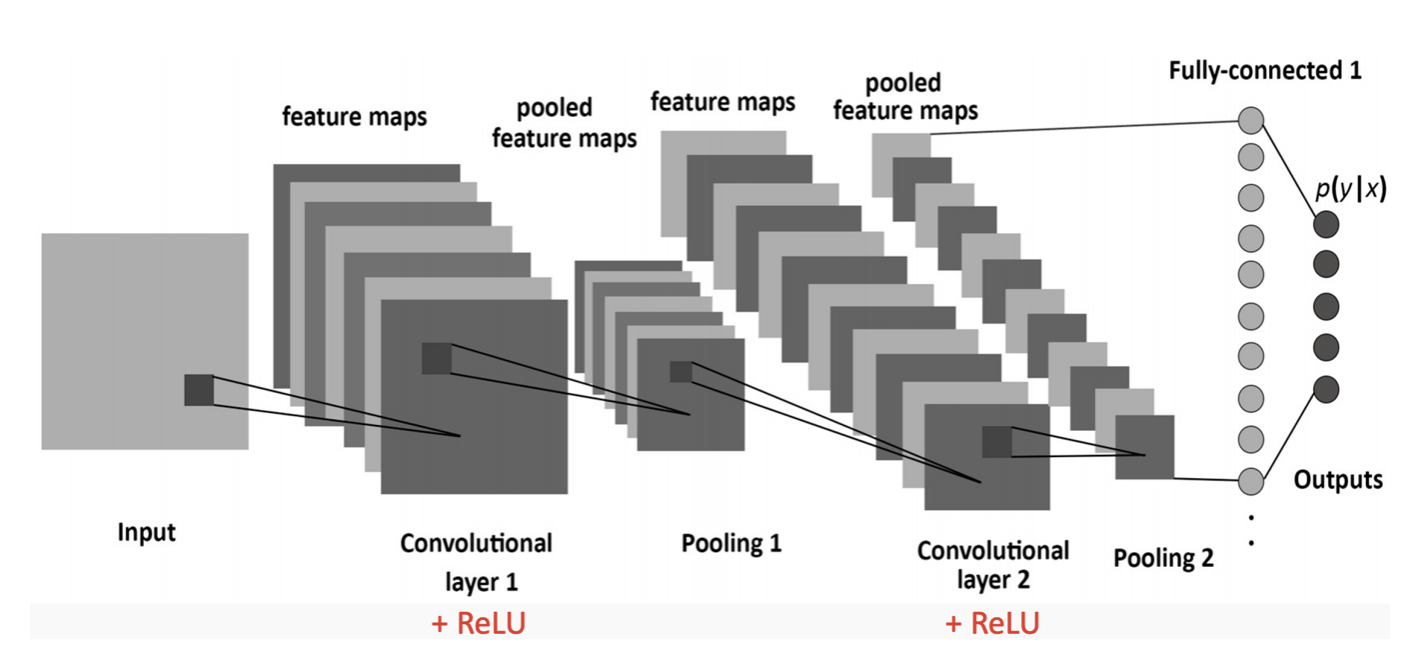
\includegraphics[scale=0.45]{Structure.png}
\caption{structure of CNN}
\end{figure}

\textbf{Convolutional Layer}\\[5]
We analyze the influence of nearby pixels in an image by using something called a filter. A filter is exactly what you think it is, in our situation, we take a filter of a size specified by the user (a rule of thumb is 3x3 or 5x5) and we move this across the image from top left to bottom right. For each point on the image, a value is calculated based on the filter using a convolution operation. For example:\\
\begin{figure}[htbp]
\centering
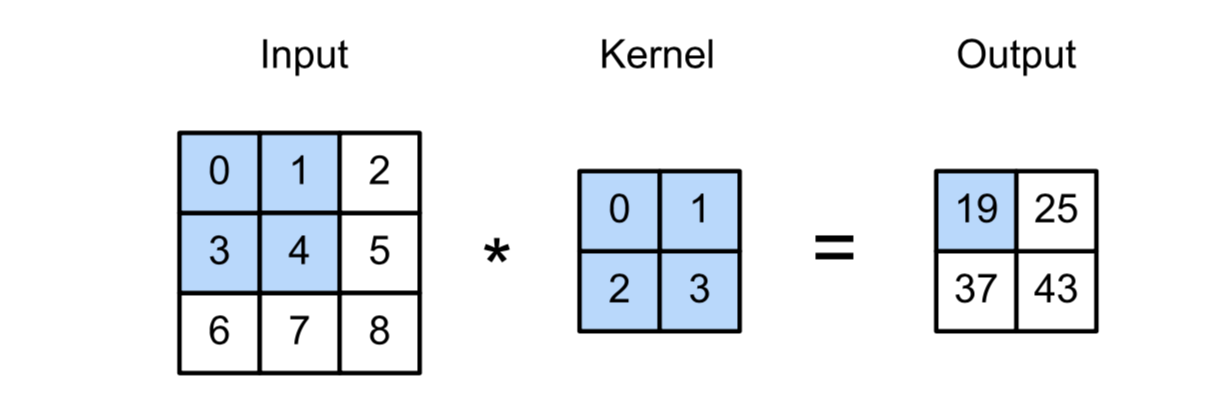
\includegraphics[width=6.5cm]{convolution.png}
\caption{processing of convolutional}
\end{figure}

In this example, the input is 3*3 and the kernel window is 2*2. we begin with the convolution window positioned at the top-left corner of the input array and slide it across the input array, both from left to right and top to bottom. When the convolution window slides to a certain position, the input subarray contained in that window and the kernel array are multiplied (element-wise) and the resulting array is summed up yielding a single scalar value. This result is precisely the value of the output array at the corresponding location.\\[2]
We could formally express this idea as follows:

$$h[i,j] = u[i,j] + \sum_{k,l} W[i,j,k,l]*x[k,l] = u[i,j] + \sum_{a,b} V[i,j,a,b]*x[i+a,j+b]$$

After the filters have passed over the image, a convolutional operation is generated for each filter. These are then taken through an activation function, for example, ReLU and Sigmoid function, which decides whether a certain feature is present at a given location in the image.\\
We can then do a lot of things, such as adding more convolutional layers, which become more and more abstract as we create a deeper CNN. \\

\textbf{Pooling Layer}\\[4]
Pooling layers could mitigating the sensitivity of convolutional layers to location and spatially downsampling representations.In theory, any type of operation can be done in pooling layers, but in practice, max pooling perform better. Here is an example of max pooling:\\
\begin{figure}[htbp]
\centering
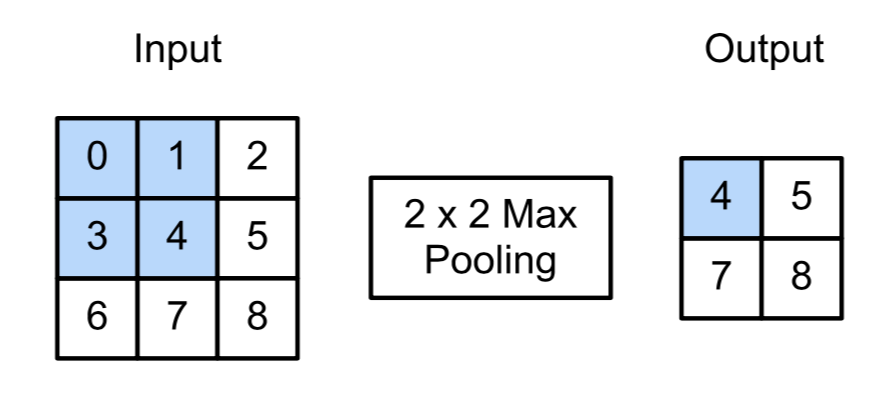
\includegraphics[width=6.5cm]{max-pooling.png}
\caption{Max pooling}
\end{figure}\\
Maximum pooling with a pooling window shape of $2*2$. The shaded portions represent the first output element and the input element used for its computation: max$(0, 1, 3, 4) = 4$\\

\textbf{Dropout}\\[4]
Deep neural nets with a large number of parameters are very powerful machine learning systems. However, overfitting is a serious problem in such networks. Large networks are also slow to use, making it difficult to deal with overfitting by combining the predictions of many different large neural nets at test time. Dropout is a technique for addressing this problem. The key idea is to randomly drop units (along with their connections) from the neural network during training. In other words, dropout with drop probability p is applied as follows:
\begin{figure}[htbp]
\centering
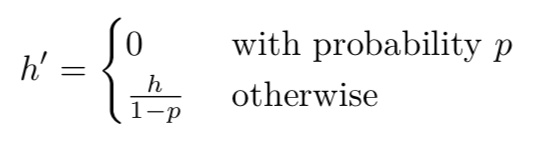
\includegraphics[scale = 0.5]{function.png}
\end{figure}


This prevents units from co-adapting too much. 


\subsection{KNN}
Altman, N. S point out that "Nonparametric regression is a collection of techniques for fitting a curve when there is little a priori knowledge about its shape." in the paper "An introduction to kernel and nearest-neighbor nonparametric regression". It shows that KNN might be a simple and useful model in our condition.\\[2]
In our project, we implement this model by sklearn. The k-nearest-neighbor classifier is commonly based on the Euclidean distance between a test sample and the specified training samples. Let xi be an input sample with p features (x$_{i1}$,x$_{i2}$,…,x$_{ip}$) , n be the total number of input samples (i=1,2,…,n) and p the total number of features (j=1,2,…,p) . The Euclidean distance between sample xi and x$_{l}$ (l=1,2,…,n) is defined as d(x$_{i}$,x$_{l}$) = $\sqrt{(x_{i1}-x_{l1})^{2} +(x_{i2}-x_{l2})^{2} + (x_{i3}-x_{l3})^{2} + ... + (x_{ip}-x_{lp})^{2}}$
In our scenario, donate K as 2. We also test with different Stop-words.
\subsection{RNN}
LSTM is an important part of RNN.Long short-term memory (LSTM) networks were discovered by Hochreiter and Schmidhuber in 1997 and set accuracy records in multiple applications domains. (Long Short-Term Memory, 1997 volume 9). \\[2]
Unlike standard feedforward neural networks, LSTM has feedback connections. It can not only process single data points (such as images), but also entire sequences of data, such as reivew text.
So, In our project, we implement LSTM with keras. We use keras. Tokenizer to transfer reviews into token. Then we embed it with Kearas embedding layer. We aslo add a layer of dropout to avoid over-fit.
\subsection{Seq2seq}
In our project, we implement this model by pytorch, and the base structure of encoder and decoder are shown as figure 6 figure 7. The first four time steps are encoder part and the other time steps are decoder part. No matter encoder or decoder, all of them are GRU model. GRUs are improved version of standard recurrent neural network. GRU (Gated Recurrent Unit) aims to solve the vanishing gradient problem which comes with a standard recurrent neural network. It can also be considered as a variation on the LSTM because both are designed similarly and, in some cases, produce equally excellent results. \\[2]
To solve the vanishing gradient problem of a standard RNN, GRU uses, so-called, update gate and reset gate. Basically, these are two vectors which decide what information should be passed to the output. The special thing about them is that they can be trained to keep information from long ago, without washing it through time or remove information which is irrelevant to the prediction. The structure of GRU is shown in figure 8.\\[2]
Update gate: help the model to determine how much of the past information (from previous time steps) needs to be passed along to the future.
$$Z_{t} = \sigma (W^{(z)}x_t + U^{(z)}h_{(t-1)})$$
Reset gate: decide how much of the past information to forget.
$$r_t = \sigma (W^{(r)}x_t + U^{(r)}h_{(t-1)})$$
Current memory content: 
$$h_t^{'} = tanh(Wx_t + r_t\odot Uh_{(t-1)})$$
Final memory at current time step: The network needs to calculate $h_t$ which holds information for the current unit and passes it down to the network. In order to do that the update gate is needed. It determines what to collect from the current memory content $h_t^{'}$ and what from the previous steps $h_(t-1)$.
$$h_t = z_t \odot h_{(t-1)} +(1-z_t)\odot h_t^{'}$$\\
\begin{figure}[h]
\centering
\begin{minipage}[t]{0.48\textwidth}
\centering
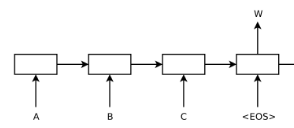
\includegraphics[width=6cm]{encoder.png}
\caption{structure of encoder}
\end{minipage}
\begin{minipage}[t]{0.48\textwidth}
\centering
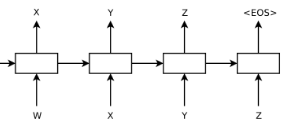
\includegraphics[width=6cm]{decoder.png}
\caption{structure of decoder}
\end{minipage}
\end{figure}\\

\begin{figure}[htb]
\centering
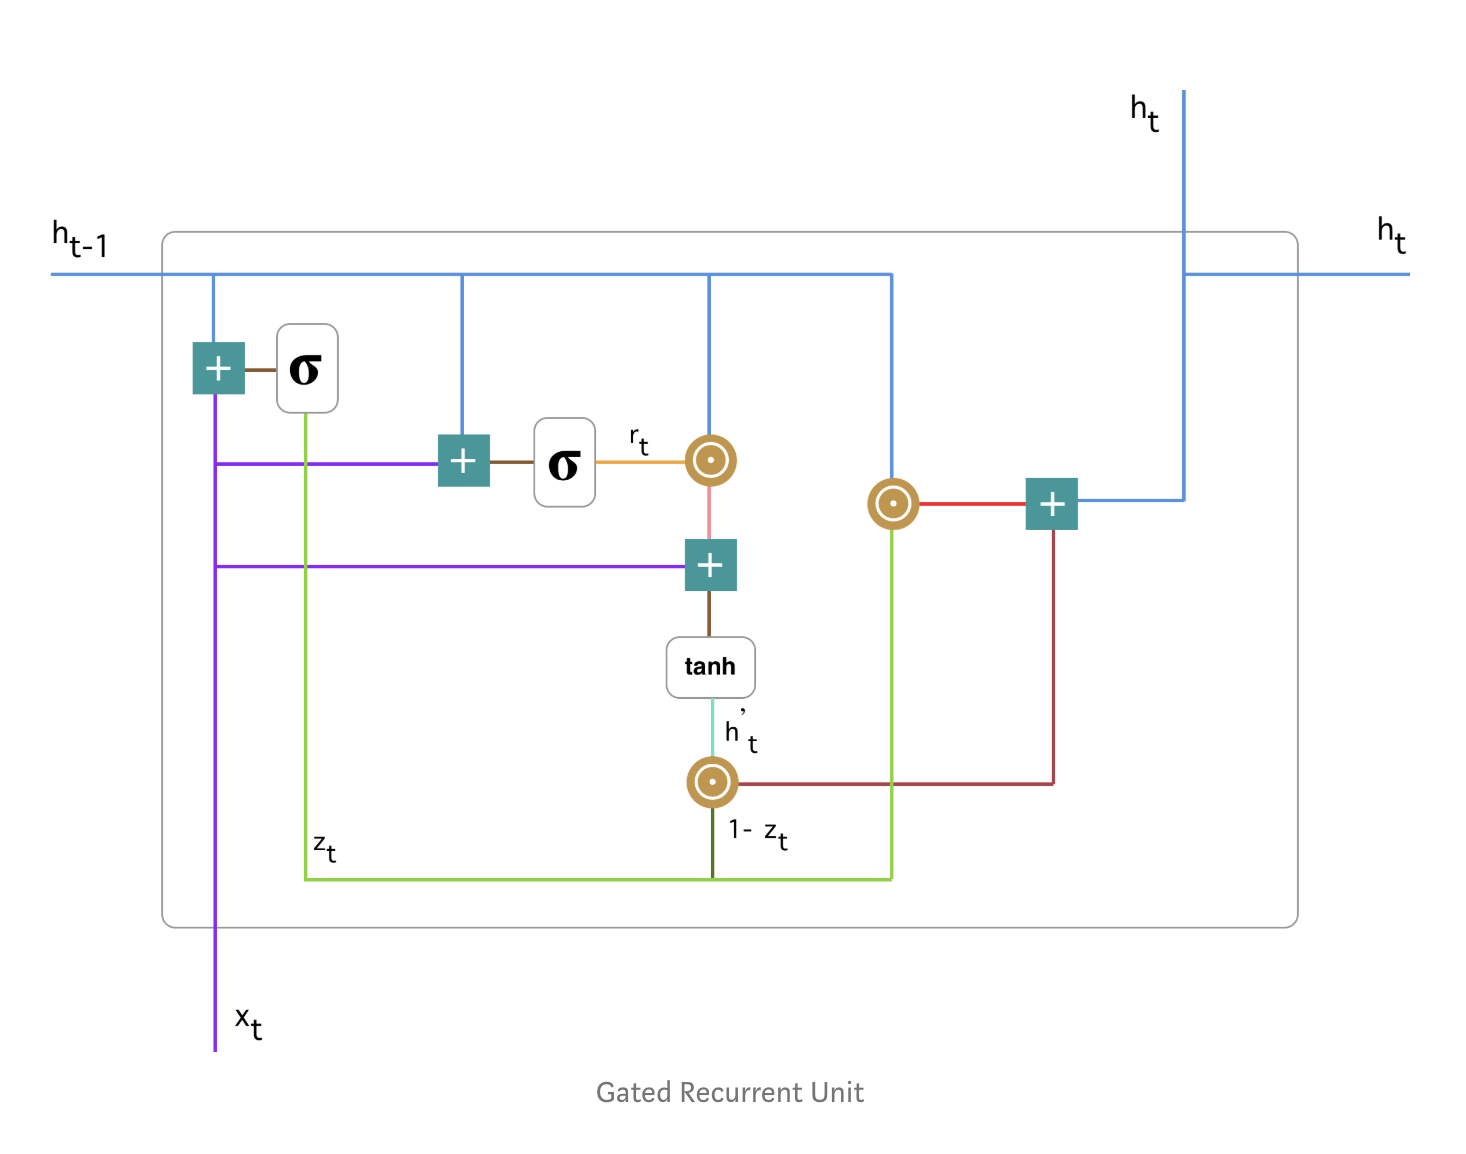
\includegraphics[width=6.5cm]{GRU.png}
\caption{structure of GRU}
\end{figure}\\


\subsection{Attention}
Attention was presented by Dzmitry Bahdanau, et al. in their paper “Neural Machine Translation by Jointly Learning to Align and Translate” that reads as a natural extension of their previous work on the Encoder-Decoder model. Instead of encoding the input sequence into a single fixed context vector, the attention model develops a context vector that is filtered specifically for each output time step. There are many main attention mechanism, and we will implement one of them.\\[2]
The structure of it is shown in figure 9. The ith Target word context vector c-i will be based on the hidden vector of each source word h-j weighted summation yields: $$C_i=\sum_{j=1}^{Tx}\alpha_{ij}h_{j}$$
For each h-j of a-ij calculated as follows:
$$\alpha_{ij} = \frac{exp(e_{ij})}{\sum_{k=1}^{Tx}(exp(e_{ik}))}$$
among them:
$$e_{ij} = a(s_{i-1},h_j)$$
$e_{ij}$ is the alignment model, representing the position j input and location i. The output matches the score of the degree based on the implied state of the i-1 position of the RNN $s_{i-1}$ dnd j position $h_{j}$ calculated.
\begin{figure}[htbp]
\centering
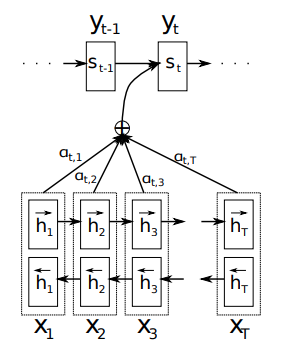
\includegraphics[scale=0.35]{bahda.png}
\caption{Structure of attention}
\end{figure}


\subsection{Teacher Forcing}
Teacher forcing is the technique where the target word is passed as the next input to the decoder. Figure 10 and figure 11 show the model with teacher forcing and without teacher forcing. Training with Teacher Forcing converges faster. At the early stages of training, the predictions of the model are very bad. If we do not use Teacher Forcing, the hidden states of the model will be updated by a sequence of wrong predictions, errors will accumulate, and it is difficult for the model to learn from that.

\begin{figure}[htbp]
\centering
\begin{minipage}[t]{0.48\textwidth}
\centering
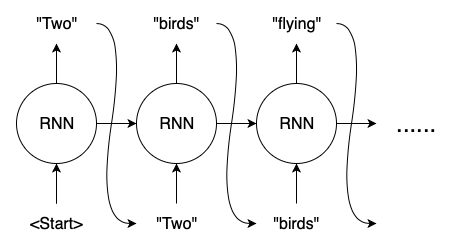
\includegraphics[width=6cm]{with_teacher_forcing.png}
\caption{without teacher forcing}
\end{minipage}
\begin{minipage}[t]{0.48\textwidth}
\centering
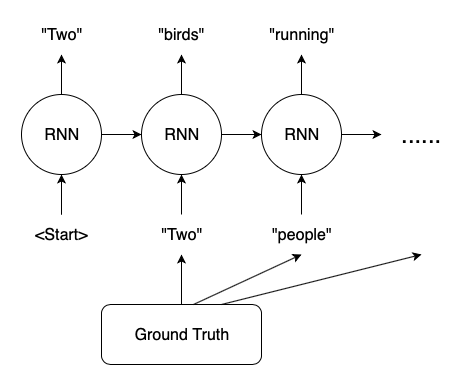
\includegraphics[width=6cm]{without_teacher_forcing.png}
\caption{with teacher forcing}
\end{minipage}
\end{figure}

\subsection{Evaluation methods}
BLEU, or the Bilingual Evaluation Understudy, is a score for comparing a candidate translation of text to one or more reference translations. Although developed for translation, it can be used to evaluate text generated for a suite of natural language processing tasks. In our project, we use BLEU score to evaluate our summarization model.

\section{Result of models}
\subsection{CNN}
In the project, we build an CNN model to predict the sentiment of these food reviews. Here is the structure of CNN model:\\
\begin{figure}[htbp]
\centering
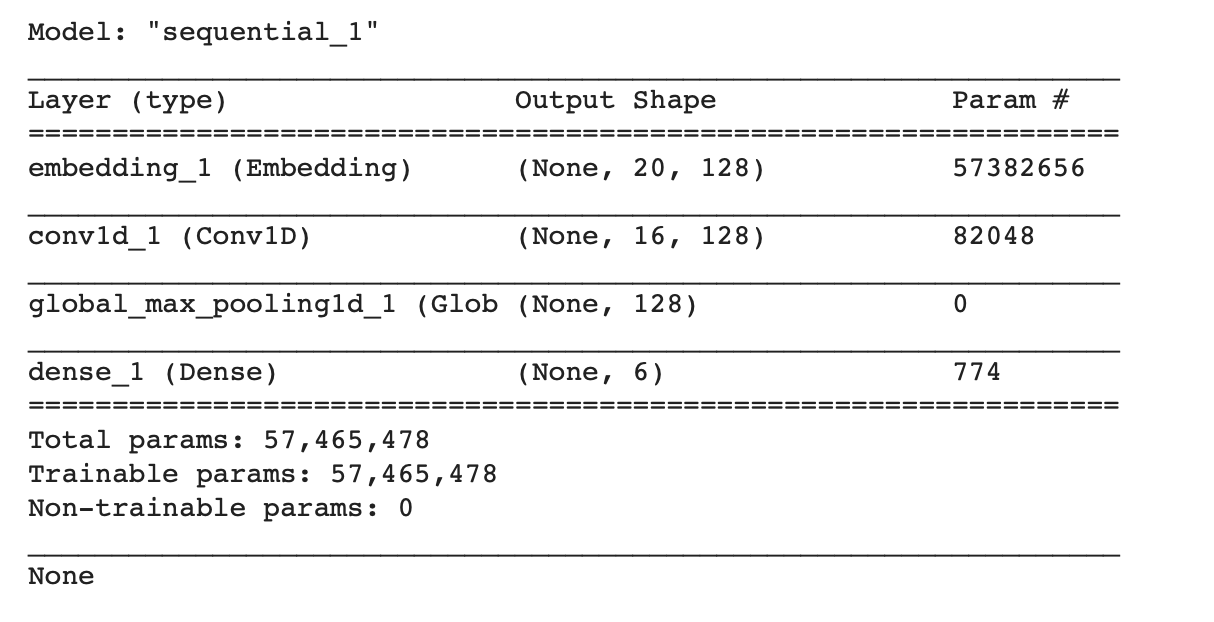
\includegraphics[scale=0.4]{stru1.png}
\end{figure}\\
At the beginning, we are confused about the standard length of food reviews. Should we choose longest length of texts or just choose the mean value of texts? Then we analyse the length of these texts. Here is the boxplot of the length of food reviews:\\
\begin{figure}[h]
\centering
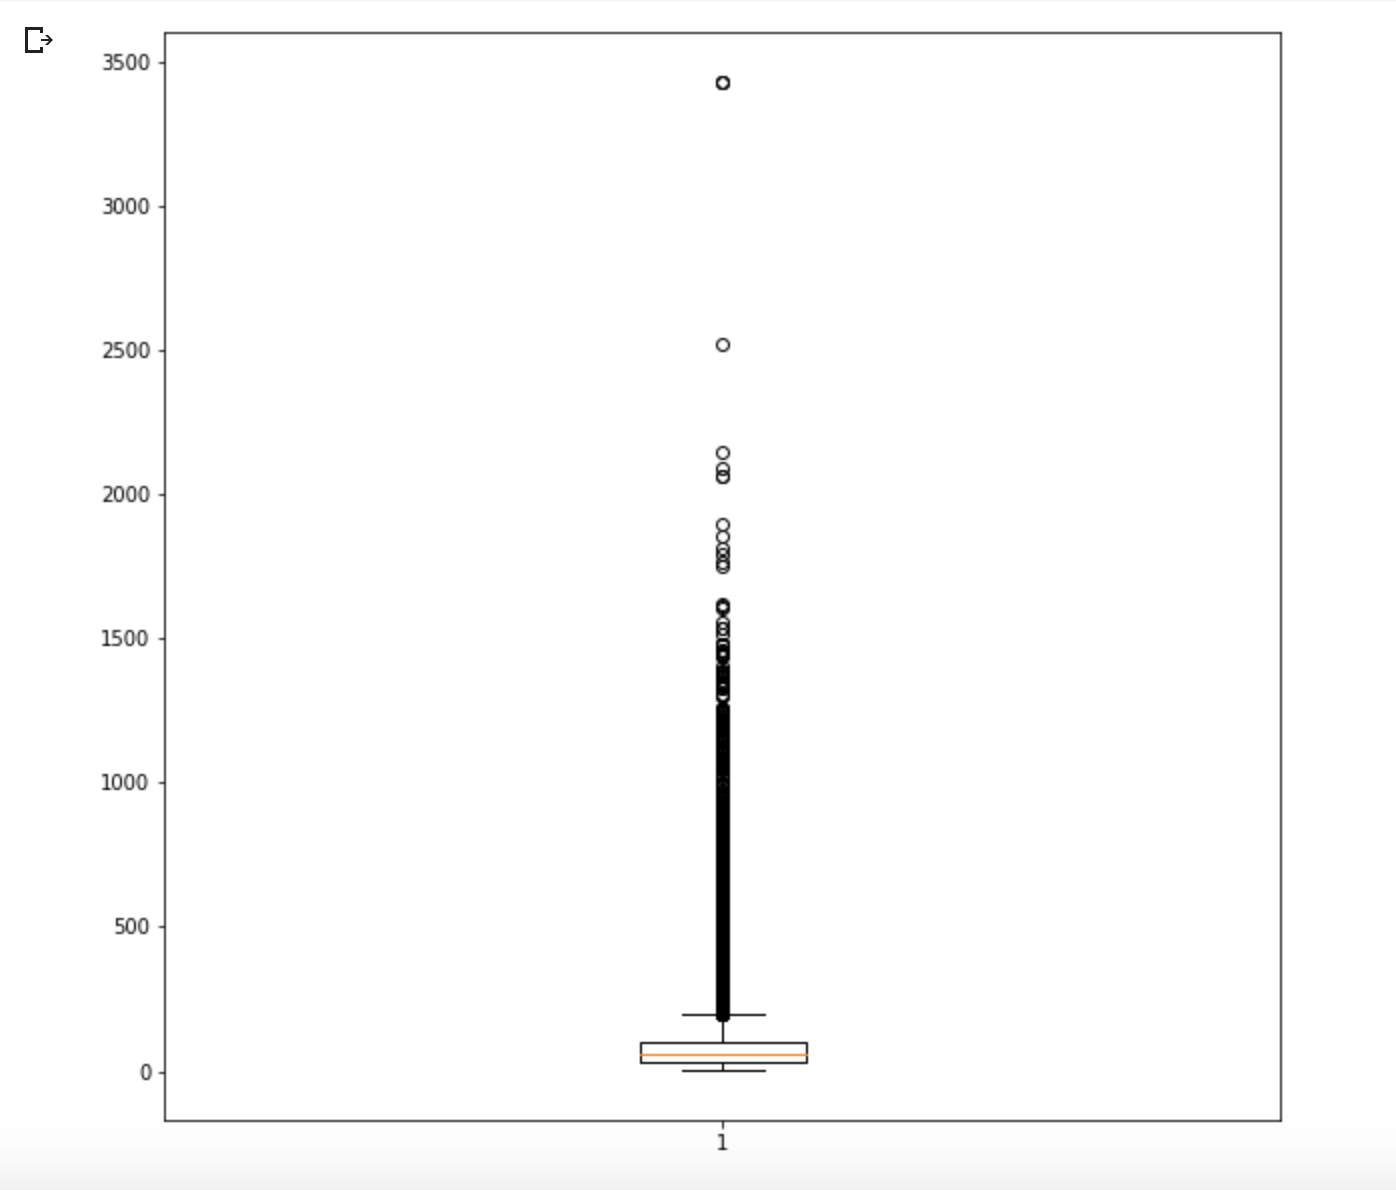
\includegraphics[width=6.5cm]{m4.png}
\caption{Length of texts}
\end{figure}\\
In the experiment, we choose two types of length of texts to see if there is the any difference in final accuracy between the mean of texts and the longest value of texts. But finally we find the accuracy of model does not improve a lot. So in the following models we just choose mean value of texts.\\
\begin{figure}[h]
\centering
\begin{minipage}[t]{0.48\textwidth}
\centering
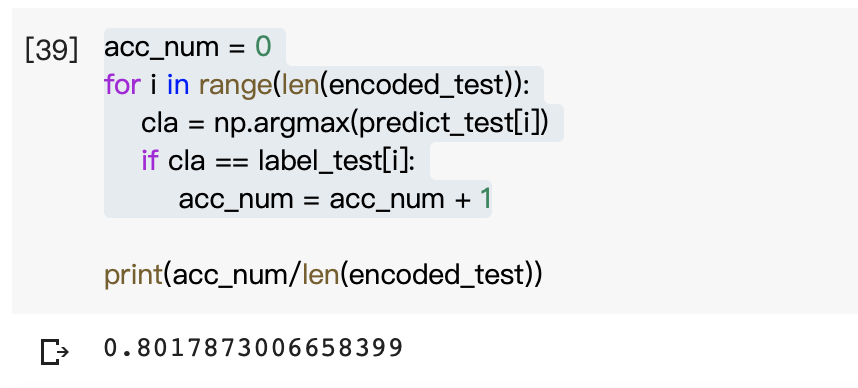
\includegraphics[width=6cm]{m3.png}
\caption{mean value of texts}
\end{minipage}
\begin{minipage}[t]{0.48\textwidth}
\centering
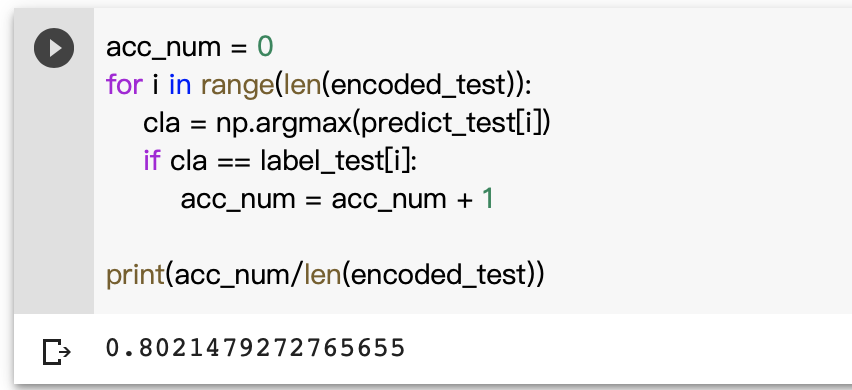
\includegraphics[width=6cm]{a3.png}
\caption{longest texts}
\end{minipage}
\end{figure}\\
We also use the "Stopword" to reduce some irrelevant words in texts in order to improve the accuracy of this model. Unfortunately, the result is not very well.\\
\begin{figure}[h]
\centering
\begin{minipage}[t]{0.48\textwidth}
\centering
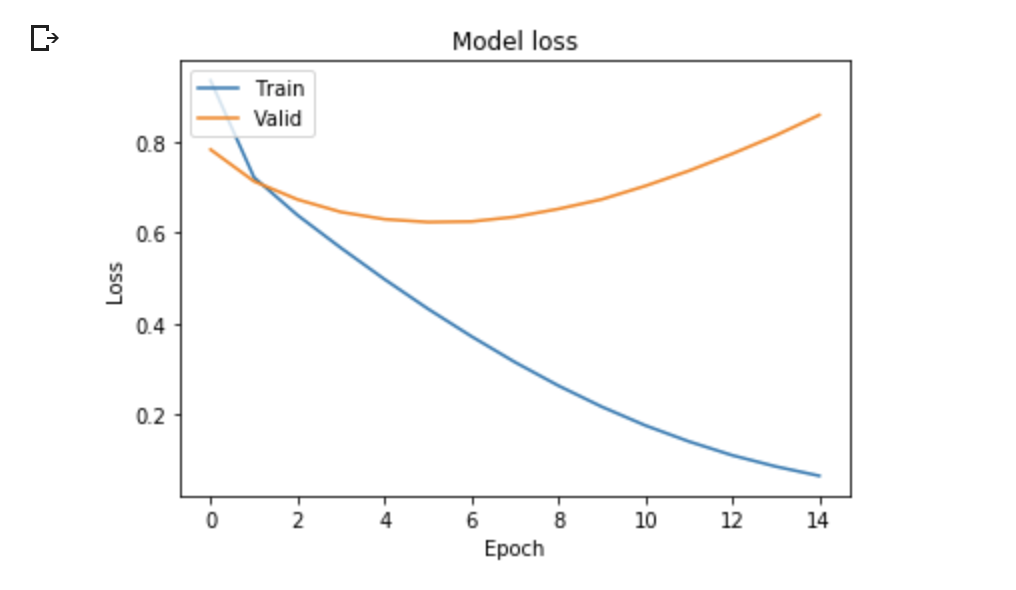
\includegraphics[width=6cm]{s4.png}
\caption{Loss}
\end{minipage}
\begin{minipage}[t]{0.48\textwidth}
\centering
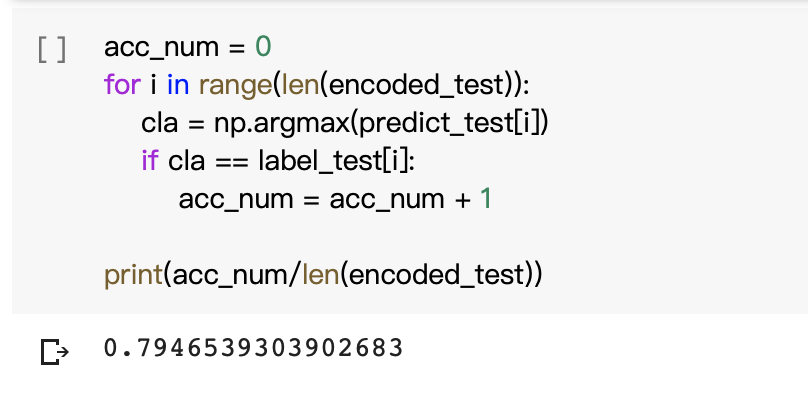
\includegraphics[width=6cm]{s2.png}
\caption{Final result}
\end{minipage}
\end{figure}

\subsection{RNN}
At first, the result is not so good. We use NLTK stopwords list as filter to eliminate stopwords. The Accuracy is not so good.

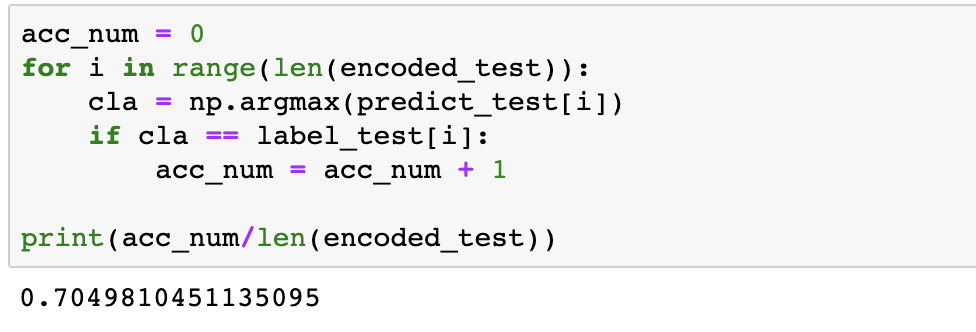
\includegraphics[width=6.5cm]{RNN_bad.png}

At first, we think it was result from the fact that we did not implement dropout. But After we add dropout, the performance still not good.\\
Then we try to improve Accuracy by changing stopwords. So, we calculated the frequency of occurrence of each stopword in the review text of error prediction. We think the words with high frequency will reduce the accuracy of our prediction. So, we created a new stopword list based on the NLTK stopword list by removing stopwords that have a high frequency of occurrence in the review text of error prediction. Luckily, it works. The accuracy increased as we remove stopwords from the stopwords list. Finally, the accuracy reaches the peak after we use an empty list as stopword list.


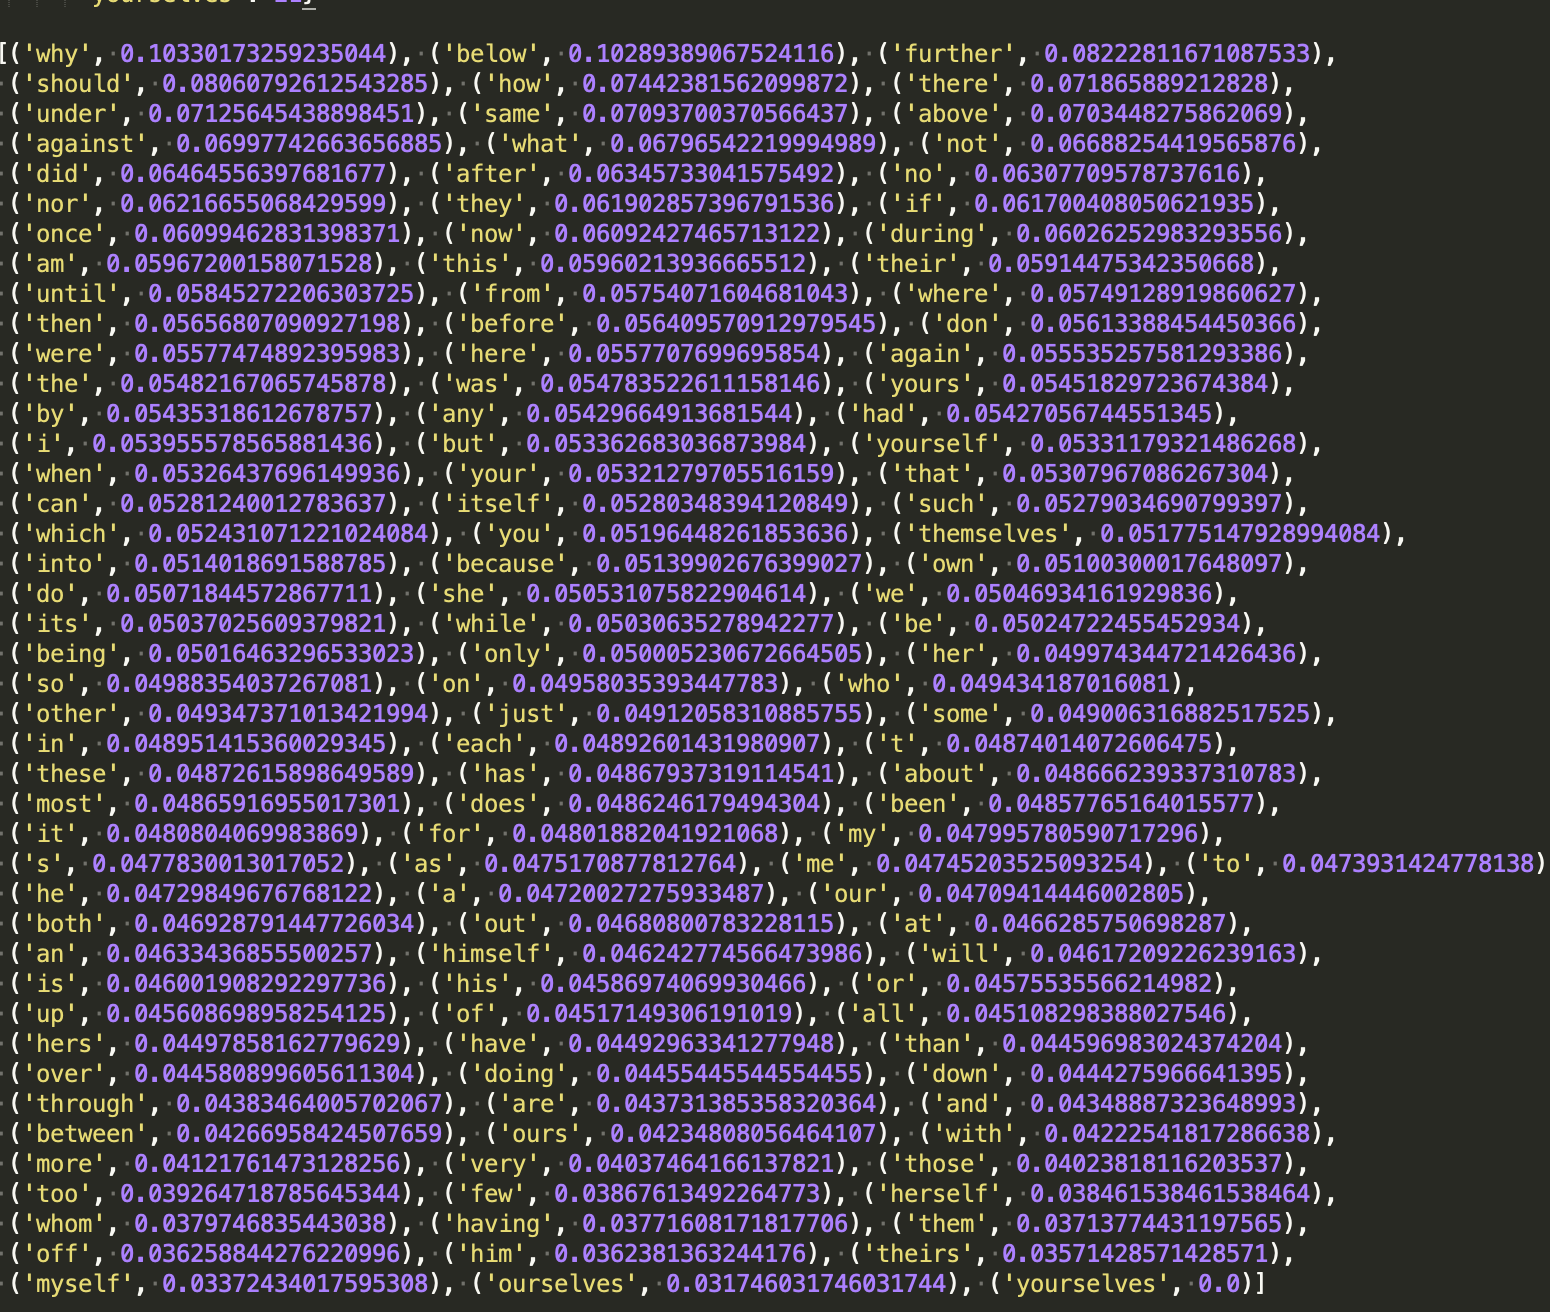
\includegraphics[width = 6.0in, height = 2.8in]{stopwords.png}

The Accuracy is 78.7080\%

\subsection{KNN}
In our project, we have implement it with NLTK stopwords list, Customized stop words, and none stopwords. We find that the less the stopwords list, the higher the accuracy is.We figure out that when we donate that K = 2 and without stopwords the performance will reach the peak. The Accuracy reach peak 77.91\%.

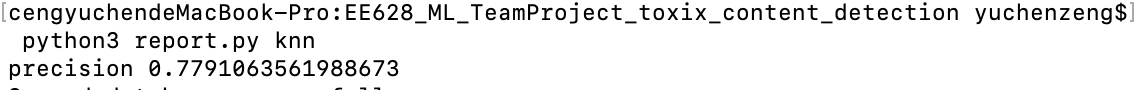
\includegraphics[scale=1]{KNN.jpg}
\subsection{seq2seq}
Loss is shown in figure 17 and the final loss is 4.36, the left column is process bar. Total BLEU score is shown in figure 18, it is 0.7, not a bad score. Finally, the total accuracy about sentiment is shown in figure 19, it is 0.83. Here are some examples about what the machine generate from original text. First two is right and the third one has different sentiment to label's sentiment which is negative.

(1). text: 13 dollars for 24 cups free shipping over 50 dollars is the going rate. These folks are pulling a swiftie.
label: beware
sum: beware<EOS>

(2). text: If your dog likes Naked bars then this is the same consistency. It's hard and sometimes my dog will eat it sometimes he'll...
label: Not happy about this
sum: Not as good as what I find <EOS>

(3). text:I ordered the ranch flavor and when I received them they had a sell by date of September of 2008!!!
label: Dont Buy!!
sum: Great Taste<EOS>

\begin{figure}
\centering
\begin{minipage}[t]{0.48\textwidth}
\centering
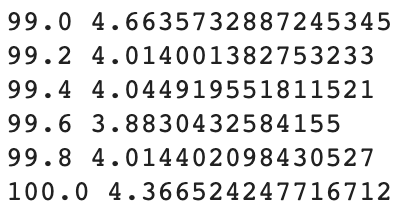
\includegraphics[width=6cm]{loss.png}
\caption{loss}
\end{minipage}
\begin{minipage}[t]{0.48\textwidth}
\centering
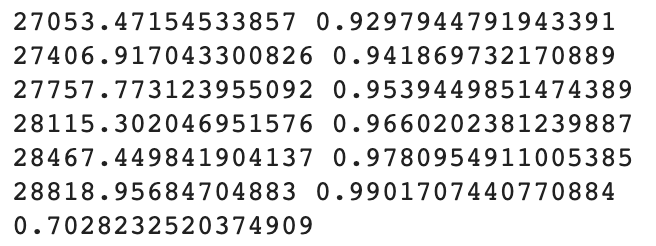
\includegraphics[width=6cm]{bleu.png}
\caption{BLEU score}
\end{minipage}
\end{figure}
\begin{figure}
    \centering
    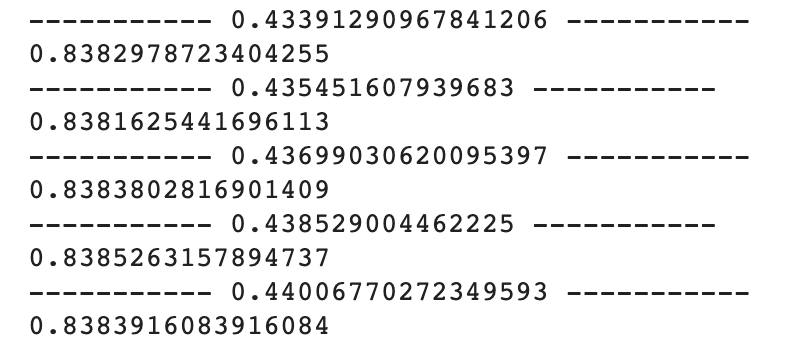
\includegraphics[width = 3.0in, height = 1.4in]{accuracy.png}
    \caption{accuracy}
    \label{fig: 9 }
\end{figure}


\section{Conclusion}
After train and test models that we mentioned previously, CNN got the best performance. RNN and KNN are little bit lower than CNN. Although seq2seq method got a better result, but it only test on a part of whole dataset.

\section{Future work}
In our project, we only set teacher forcing parameter is 0.5 which means not all the time steps use ground truth. In other words, we can try to find a better ratio of it to get better performance.

Another thing is, we can implement beam search in NLG process which can generate better sentences.
\section*{References}

[1] Minh-Thang Luong.\ \& Hieu Pham\ \& Christopher D. Manning(2015) Effective Approaches to Attention-based Neural Machine Translation. Computer Science Department, Stanford University, Stanford, CA 94305

[2] Dzmitry Bahdanau\ \& KyungHyun Cho\ \& Yoshua Bengio(2016) neural machine translation by jointly learning to align and translate.

[3] Kishore Papineni, Salim Roukos\ \& Todd Ward\ (2002) BLEU: a Method for Automatic Evaluation of Machine Translation. IBM T. J. Watson Research Center Yorktown Heights, NY 10598, USA

[4] Hochreiter, Sepp; Schmidhuber, Jürgen (1997-11-01). "Long Short-Term Memory". Neural Computation.

[5] Altman, N. S. (1992). "An introduction to kernel and nearest-neighbor nonparametric regression". The American Statistician. 46 (3): 175–185. 



\end{document}
